\documentclass[12pt,a4paper]{report}
\usepackage[utf8]{vietnam}
\usepackage{amsmath}
\usepackage{amsfonts}
\usepackage{amssymb}
\usepackage{graphicx}
\usepackage{hyperref}
\usepackage{listings}
\usepackage{xcolor}
\usepackage{geometry}
\usepackage{fancyhdr}
\usepackage{titlesec}
\usepackage{booktabs}
\usepackage{array}
\usepackage{longtable}
\usepackage{enumitem}
\usepackage{adjustbox}
\usepackage{url}
\usepackage{xurl}

\geometry{left=3.5cm,right=2cm,top=3cm,bottom=2.5cm}

% Macro để hiển thị JSON với ngắt dòng tự động
\newcommand{\json}[1]{\texttt{\allowbreak#1\allowbreak}}

% Cấu hình code listing
\lstset{
    language=C,
    basicstyle=\ttfamily\footnotesize,
    keywordstyle=\color{blue}\bfseries,
    commentstyle=\color{green!60!black},
    stringstyle=\color{red},
    numbers=left,
    numberstyle=\tiny\color{gray},
    stepnumber=1,
    numbersep=5pt,
    frame=single,
    breaklines=true,
    showstringspaces=false,
    tabsize=2
}

% Cấu hình hyperref
\hypersetup{
    colorlinks=true,
    linkcolor=blue,
    filecolor=magenta,      
    urlcolor=cyan,
    pdftitle={Báo cáo cuối kỳ - Ứng dụng thi trắc nghiệm online},
    pdfauthor={Hoàng Kim Trí Thành, Dương Trung Kiên, Lường Hải Đăng}
}

% Header và Footer
\pagestyle{fancy}
\fancyhf{}
\fancyhead[L]{\leftmark}
\fancyhead[R]{\thepage}
\fancyfoot[C]{Báo cáo cuối kỳ - Thực hành Lập trình Mạng}

\titleformat{\chapter}[display]
{\normalfont\huge\bfseries}{\chaptertitlename\ \thechapter}{20pt}{\Huge}

\begin{document}

% Trang bìa
\begin{titlepage}
    \centering
    \vspace*{0.2cm}
    
    {\LARGE\bfseries ĐẠI HỌC BÁCH KHOA HÀ NỘI}\\
    \vspace{0.2cm}
    {\large TRƯỜNG CÔNG NGHỆ THÔNG TIN VÀ TRUYỀN THÔNG}\\
    \vspace{0.3cm}
    
    % Logo Đại học Bách Khoa
    
\includegraphics[width=3cm]{images/Logo_Đại_học_Bách_Khoa_Hà_Nội.svg.png}
    \vspace{0.4cm}
    
    \rule{\textwidth}{1pt}
    \vspace{0.3cm}
    
    {\Huge\bfseries BÁO CÁO CUỐI KỲ}\\
    \vspace{0.3cm}
    {\Large\bfseries MÔN: THỰC HÀNH LẬP TRÌNH MẠNG}\\
    \vspace{0.3cm}
    \rule{\textwidth}{1pt}
    \vspace{0.8cm}
    
    {\LARGE\bfseries ĐỀ TÀI:}\\
    \vspace{0.3cm}
    {\Large\bfseries XÂY DỰNG ỨNG DỤNG THI TRẮC NGHIỆM ONLINE}\\
    \vspace{1cm}
    
    \begin{flushleft}
        \large
        \textbf{Nhóm thực hiện:}\\
        \vspace{0.15cm}
        Hoàng Kim Trí Thành - MSSV: 20210798\\
        Dương Trung Kiên - MSSV: 20215067\\
        Lường Hải Đăng - MSSV: 20210151\\
        \vspace{0.5cm}
        \textbf{Giảng viên hướng dẫn:} PGS.TS. Trương Thị Diệu Linh\\
        \vspace{0.25cm}
        \textbf{Thời gian:} Học kì 20251
    \end{flushleft}
    
    \vfill
    
    {\large Hà Nội, \today}
    
\end{titlepage}

% Mục lục
\tableofcontents
\newpage
\listoffigures
\newpage
\listoftables

% Nội dung chính
\chapter{Tổng quan}

\section{Giới thiệu đề tài}

Trong thời đại công nghệ số hiện nay, việc áp dụng công nghệ thông tin vào giáo dục đã trở thành xu hướng tất yếu. Hệ thống thi trắc nghiệm online là một trong những ứng dụng quan trọng, giúp tối ưu hóa quá trình đánh giá và kiểm tra kiến thức của học sinh, sinh viên.

Đề tài "Xây dựng ứng dụng thi trắc nghiệm online" được thực hiện nhằm phát triển một hệ thống quản lý thi cử hoàn chỉnh với đầy đủ các chức năng: quản lý người dùng, quản lý lớp học, quản lý đề thi, tổ chức thi trực tuyến, chấm điểm tự động và xử lý khiếu nại.

\section{Mục tiêu của đề tài}

\begin{itemize}
    \item Xây dựng hệ thống thi trắc nghiệm online với kiến trúc Client-Server
    \item Phát triển Backend Server sử dụng C Socket Programming với giao thức TCP/IP
    \item Phát triển Frontend Client sử dụng Qt Framework với giao diện đồ họa thân thiện
    \item Tích hợp MySQL Database để lưu trữ dữ liệu
    \item Triển khai các chức năng quản lý lớp học, đề thi, người dùng
    \item Hỗ trợ thi trực tuyến với timer và chấm điểm tự động
    \item Xây dựng hệ thống phân quyền (Admin, Teacher, Student)
\end{itemize}

\section{Phạm vi ứng dụng}

Hệ thống được thiết kế để phục vụ:
\begin{itemize}
    \item \textbf{Quản trị viên (Admin):} Quản lý người dùng, duyệt tài khoản, phân quyền
    \item \textbf{Giáo viên (Teacher):} Tạo lớp học, quản lý sinh viên, tạo đề thi, xem kết quả, xử lý khiếu nại
    \item \textbf{Sinh viên (Student):} Tham gia lớp học, làm bài thi, luyện tập, xem kết quả, gửi khiếu nại
\end{itemize}

\chapter{Phân tích và thiết kế hệ thống}

\section{Phân tích yêu cầu}

\subsection{Yêu cầu chức năng}

Hệ thống cần đáp ứng các yêu cầu chức năng sau:

\subsubsection{Quản lý người dùng}
\begin{itemize}
    \item Đăng ký tài khoản mới
    \item Đăng nhập vào hệ thống
    \item Phân quyền người dùng (Admin, Teacher, Student)
    \item Duyệt tài khoản mới (dành cho Admin)
    \item Quản lý thông tin người dùng
\end{itemize}

\subsubsection{Quản lý lớp học}
\begin{itemize}
    \item Tạo lớp học mới (Teacher)
    \item Xem danh sách lớp học
    \item Xem chi tiết lớp học
    \item Thêm/xóa sinh viên vào lớp (Teacher)
    \item Quản lý thành viên lớp
\end{itemize}

\subsubsection{Quản lý đề thi}
\begin{itemize}
    \item Tạo đề thi mới
    \item Ngân hàng câu hỏi
    \item Thêm/sửa/xóa câu hỏi
    \item Quản lý đề thi (draft, published)
    \item Bắt đầu/kết thúc kỳ thi
\end{itemize}

\subsubsection{Thi trực tuyến}
\begin{itemize}
    \item Tham gia kỳ thi
    \item Giao diện làm bài với timer
    \item Lưu câu trả lời
    \item Nộp bài và chấm điểm tự động
    \item Xem kết quả thi
\end{itemize}

\subsubsection{Chế độ luyện tập}
\begin{itemize}
    \item Làm bài luyện tập không giới hạn
    \item Random câu hỏi từ ngân hàng
    \item Xem đáp án ngay sau khi làm xong
\end{itemize}

\subsubsection{Khiếu nại điểm}
\begin{itemize}
    \item Sinh viên gửi khiếu nại
    \item Giáo viên xem xét và phản hồi
    \item Cập nhật điểm sau khi xử lý
\end{itemize}

\subsubsection{Thống kê}
\begin{itemize}
    \item Thống kê điểm số theo lớp
    \item Thống kê điểm số theo đề thi
    \item Phân bố điểm
    \item Biểu đồ thống kê
\end{itemize}

\subsection{Yêu cầu phi chức năng}

Về \textbf{hiệu năng}, hệ thống được thiết kế để hỗ trợ nhiều client kết nối đồng thời thông qua việc sử dụng multi-threading, đảm bảo phản hồi nhanh và ổn định. Về \textbf{bảo mật}, hệ thống áp dụng cơ chế phân quyền truy cập nghiêm ngặt và xác thực người dùng để đảm bảo tính bảo mật dữ liệu. \textbf{Độ tin cậy} được đảm bảo thông qua các cơ chế xử lý lỗi toàn diện và hệ thống logging chi tiết để theo dõi và khắc phục sự cố. Hệ thống được xây dựng với \textbf{khả năng mở rộng} cao nhờ kiến trúc module, cho phép dễ dàng thêm các tính năng mới mà không ảnh hưởng đến phần còn lại. Cuối cùng, \textbf{khả năng sử dụng} được tối ưu hóa thông qua giao diện đồ họa thân thiện và trực quan, giúp người dùng dễ dàng sử dụng hệ thống mà không cần đào tạo phức tạp.

\section{Thiết kế kiến trúc hệ thống}

\subsection{Kiến trúc tổng quan}

Hệ thống được xây dựng theo mô hình Client-Server với kiến trúc 3 tầng:

\begin{enumerate}
    \item \textbf{Tầng Presentation (Frontend):} Ứng dụng Qt C++ cung cấp giao diện người dùng
    \item \textbf{Tầng Business Logic (Backend):} Server C Socket xử lý logic nghiệp vụ
    \item \textbf{Tầng Data (Database):} MySQL lưu trữ dữ liệu
\end{enumerate}

\begin{figure}[h]
    \centering
    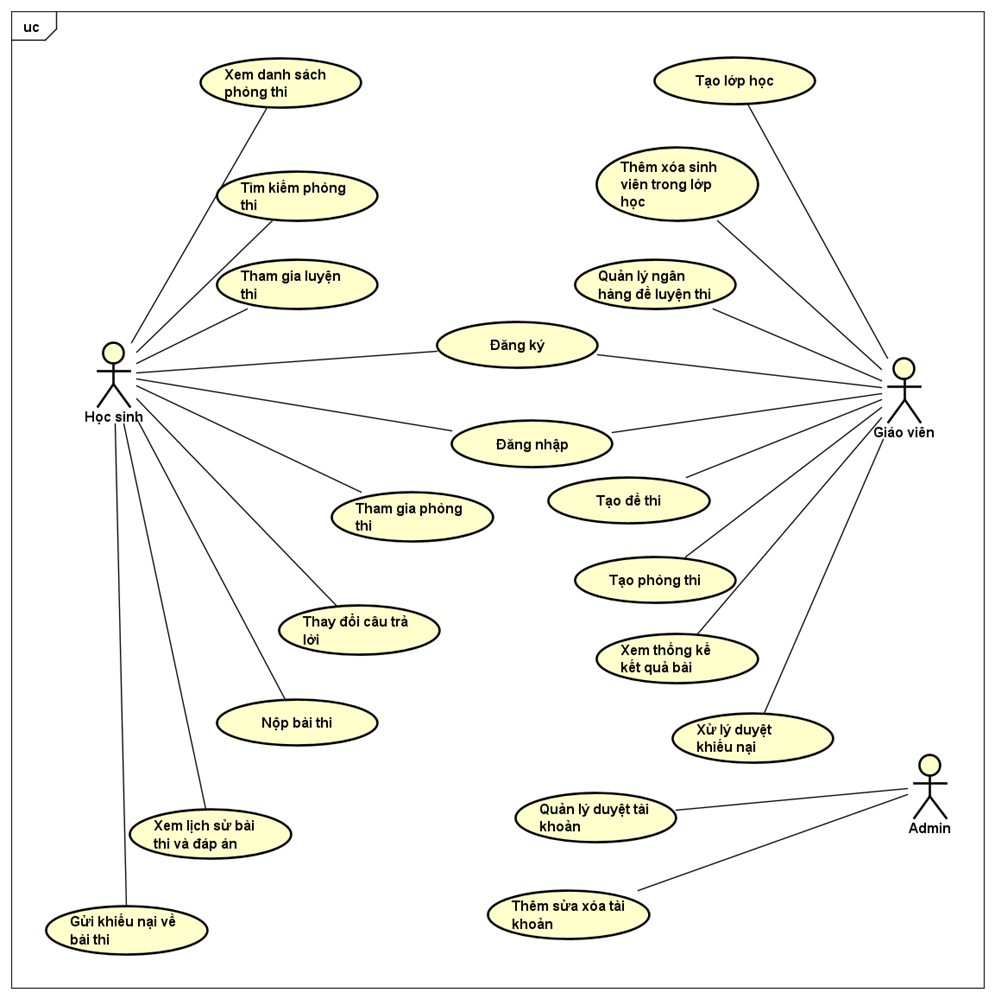
\includegraphics[width=0.8\textwidth]{images/bieudousecase.png}
    \caption{Sơ đồ kiến trúc hệ thống}
    \label{fig:architecture}
\end{figure}

\subsection{Công nghệ sử dụng}

\subsubsection{Backend Server}
\begin{itemize}
    \item \textbf{Ngôn ngữ:} C (C99)
    \item \textbf{Giao thức:} TCP/IP Socket Programming
    \item \textbf{Threading:} POSIX Threads (pthread)
    \item \textbf{Database:} MySQL C API
    \item \textbf{JSON:} cJSON library
    \item \textbf{Platform:} Linux/WSL
\end{itemize}

\subsubsection{Frontend Client}
\begin{itemize}
    \item \textbf{Ngôn ngữ:} C++
    \item \textbf{Framework:} Qt 6 (Qt Widgets)
    \item \textbf{Network:} QTcpSocket
    \item \textbf{Data Format:} JSON
    \item \textbf{Platform:} Cross-platform (Windows, Linux, macOS)
\end{itemize}

\subsubsection{Database}
\begin{itemize}
    \item \textbf{Hệ quản trị:} MySQL 8.0+
    \item \textbf{Encoding:} UTF-8
    \item \textbf{Storage Engine:} InnoDB
\end{itemize}

\subsection{Sơ đồ luồng dữ liệu}

Quá trình giao tiếp giữa Client và Server diễn ra theo các bước sau:

\begin{enumerate}
    \item Client kết nối đến Server qua TCP Socket (Port 8081)
    \item Client gửi request dạng JSON với header định dạng
    \item Server nhận request, parse header và body
    \item Server xử lý logic nghiệp vụ, truy vấn database
    \item Server gửi response về Client dạng JSON
    \item Client nhận response và cập nhật giao diện
\end{enumerate}

\section{Thiết kế database}

\subsection{Mô hình dữ liệu}

Hệ thống sử dụng 13 bảng chính trong database:

\begin{enumerate}
    \item \texttt{user} - Lưu trữ thông tin người dùng
    \item \texttt{class} - Lưu trữ thông tin lớp học
    \item \texttt{user\_in\_class} - Quan hệ nhiều-nhiều giữa user và class
    \item \texttt{questions} - Ngân hàng câu hỏi
    \item \texttt{exam} - Thông tin đề thi
    \item \texttt{exam\_questions} - Quan hệ nhiều-nhiều giữa exam và questions
    \item \texttt{exam\_submissions} - Bài nộp của sinh viên
    \item \texttt{exam\_answers} - Câu trả lời chi tiết
    \item \texttt{practice\_sessions} - Phiên luyện tập
    \item \texttt{practice\_answers} - Câu trả lời luyện tập
    \item \texttt{appeals} - Khiếu nại điểm
    \item \texttt{log} - Nhật ký hoạt động hệ thống
\end{enumerate}

\subsection{Sơ đồ ER (Entity Relationship)}

Các bảng chính và quan hệ:

\begin{itemize}
    \item \texttt{user} (1) $\leftrightarrow$ (N) \texttt{user\_in\_class} $\leftrightarrow$ (N) \texttt{class}
    \item \texttt{class} (1) $\leftrightarrow$ (N) \texttt{exam}
    \item \texttt{exam} (N) $\leftrightarrow$ (N) \texttt{questions} (qua \texttt{exam\_questions})
    \item \texttt{user} (1) $\leftrightarrow$ (N) \texttt{exam\_submissions}
    \item \texttt{exam\_submissions} (1) $\leftrightarrow$ (N) \texttt{exam\_answers}
    \item \texttt{user} (1) $\leftrightarrow$ (N) \texttt{appeals}
\end{itemize}

\section{Thiết kế giao thức}

\subsection{Định dạng message}

Hệ thống sử dụng 3 loại message chính:

\subsubsection{CONTROL Message}
Format: \texttt{CONTROL <TYPE>\\n<JSON\_BODY>}

Ví dụ:
\begin{lstlisting}
CONTROL LOGIN
{"email":"student@test.com","password":"123456"}
\end{lstlisting}

\subsubsection{DATA Message}
Format: \texttt{DATA <TYPE> <DATA\_TYPE> <SIZE>\\n<JSON\_BODY>}

\subsubsection{NOTIFICATION Message}
Format: \texttt{NOTIFICATION <TYPE> <TIMESTAMP>\\n<JSON\_BODY>}

Ví dụ:
\begin{lstlisting}
NOTIFICATION LOGIN_SUCCESS 2024-01-15T10:30:00
{"user_id":1,"role":"student","name":"Nguyen Van A"}
\end{lstlisting}

\subsection{Danh sách cấu trúc gói tin}

\sloppy
\subsubsection{Authentication}
\begin{itemize}
    \item \texttt{LOGIN} - Đăng nhập \\
    Request body: \json{\{ "email": "student@test.com", "password": "123456" \}} \\
    Response: \json{\{ "user\_id": 1, "role": "student", "unread\_appeals\_count": 0 \}}
    \item \texttt{SIGN\_UP} - Đăng ký \\
    Request body: \json{\{ "email": "student@test.com", "password": "123456", "name": "Nguyen Van A", "dob": "2000-01-01" \}} \\
    Response: \json{\{ "status": "success", "message": "Sign up successful", "data": \{ "user\_id": 101 \} \}}
\end{itemize}

\subsubsection{Class Management}
\begin{itemize}
    \item \texttt{CREATE\_CLASS} - Tạo lớp học \\
    Request body: \json{\{ "class\_name": "Lớp 10A1", "description": "Mô tả lớp học", "teacher\_id": 1 \}} \\
    Response: \json{\{ "status": "success", "message": "Class created", "data": \{ "class\_id": 1, "class\_name": "Lớp 10A1", "total\_students": 5 \} \}}
    \item \texttt{GET\_CLASS\_LIST} - Lấy danh sách lớp \\
    Request body: \json{\{\}} \\
    Response: \json{\{ "data": [\{ "id": 1, "class\_name": "Lớp 10A1", "teacher\_id": 1 \}] \}}
    \item \texttt{GET\_CLASS\_DETAIL} - Chi tiết lớp \\
    Request body: \json{\{ "class\_id": 1 \}} \\
    Response: \json{\{ "data": \{ "id": 1, "class\_name": "Lớp 10A1", "description": "Mô tả", "teacher\_id": 1 \} \}}
    \item \texttt{ADD\_STUDENT\_TO\_CLASS} - Thêm sinh viên \\
    Request body: \json{\{ "class\_id": 1, "student\_id": 5 \}} \\
    Response: \json{\{ "status": "success", "message": "Student added to class" \}}
    \item \texttt{REMOVE\_STUDENT\_FROM\_CLASS} - Xóa sinh viên \\
    Request body: \json{\{ "class\_id": 1, "student\_id": 5 \}} \\
    Response: \json{\{ "status": "success", "message": "Student removed from class" \}}
    \item \texttt{GET\_MY\_CLASSES} - Lấy lớp của user \\
    Request body: \json{\{ "user\_id": 1, "role": "teacher" \}} \\
    Response: \json{\{ "data": [\{ "id": 1, "class\_name": "Lớp 10A1" \}] \}}
\end{itemize}

\subsubsection{Exam Management}
\begin{itemize}
    \item \texttt{CREATE\_EXAM} - Tạo đề thi \\
    Request body: \json{\{ "exam\_name": "Kiểm tra giữa kỳ", "description": "Mô tả đề thi", "class\_id": 1, "time\_limit": 60, "start\_time": "2024-01-15 08:00:00", "end\_time": "2024-01-15 10:00:00" \}} \\
    Response: \json{\{ "status": "success", "message": "Exam created successfully", "exam\_id": 1 \}}
    \item \texttt{GET\_EXAMS\_IN\_CLASS} - Lấy danh sách đề thi \\
    Request body: \json{\{ "class\_id": 1 \}} \\
    Response: \json{\{ "data": [\{ "id": 1, "exam\_name": "Kiểm tra giữa kỳ", "status": "draft" \}] \}}
    \item \texttt{GET\_EXAM\_DETAIL} - Chi tiết đề thi \\
    Request body: \json{\{ "exam\_id": 1 \}} \\
    Response: \json{\{ "data": \{ "id": 1, "exam\_name": "Kiểm tra giữa kỳ", "time\_limit": 60, "status": "published" \} \}}
    \item \texttt{UPDATE\_EXAM\_STATUS} - Cập nhật trạng thái \\
    Request body: \json{\{ "exam\_id": 1, "status": "published" \}} \\
    Response: \json{\{ "status": "success", "message": "Exam status updated" \}}
    \item \texttt{START\_EXAM} - Bắt đầu kỳ thi \\
    Request body: \json{\{ "exam\_id": 1 \}} \\
    Response: \json{\{ "status": "success", "message": "Exam started" \}}
    \item \texttt{JOIN\_EXAM} - Tham gia kỳ thi \\
    Request body: \json{\{ "exam\_id": 1, "user\_id": 5 \}} \\
    Response: \json{\{ "status": "success", "message": "Joined exam successfully", "submission\_id": 10 \}}
    \item \texttt{GET\_EXAM\_FOR\_STUDENT} - Lấy đề cho sinh viên \\
    Request body: \json{\{ "exam\_id": 1, "user\_id": 5 \}} \\
    Response: \json{\{ "data": \{ "exam\_id": 1, "questions": [\{ "id": 1, "question\_text": "Câu hỏi 1", "options": ["A", "B", "C", "D"] \}] \} \}}
    \item \texttt{SUBMIT\_ANSWER} - Nộp câu trả lời \\
    Request body: \json{\{ "submission\_id": 10, "question\_id": 1, "answer": "A" \}} \\
    Response: \json{\{ "status": "success", "message": "Answer submitted" \}}
    \item \texttt{SUBMIT\_EXAM} - Nộp bài \\
    Request body: \json{\{ "submission\_id": 10 \}} \\
    Response: \json{\{ "status": "success", "message": "Exam submitted", "score": 8.5, "total\_score": 10 \}}
    \item \texttt{GET\_EXAM\_RESULT} - Xem kết quả \\
    Request body: \json{\{ "submission\_id": 10 \}} \\
    Response: \json{\{ "data": \{ "submission\_id": 10, "score": 8.5, "total\_score": 10, "answers": [\{ "question\_id": 1, "user\_answer": "A", "correct\_answer": "B", "is\_correct": false \}] \} \}}
\end{itemize}

\subsubsection{Question Management}
\begin{itemize}
    \item \texttt{ADD\_QUESTION\_TO\_BANK} - Thêm câu hỏi \\
    Request body: \json{\{ "question\_text": "Câu hỏi 1?", "option\_a": "Đáp án A", "option\_b": "Đáp án B", "option\_c": "Đáp án C", "option\_d": "Đáp án D", "correct\_answer": "A" \}} \\
    Response: \json{\{ "status": "success", "message": "Question added", "question\_id": 1 \}}
    \item \texttt{GET\_QUESTION\_BANK} - Lấy ngân hàng câu hỏi \\
    Request body: \json{\{\}} \\
    Response: \json{\{ "data": [\{ "id": 1, "question\_text": "Câu hỏi 1?", "correct\_answer": "A" \}] \}}
    \item \texttt{ADD\_EXAM\_QUESTION} - Thêm câu vào đề \\
    Request body: \json{\{ "exam\_id": 1, "question\_id": 1 \}} \\
    Response: \json{\{ "status": "success", "message": "Question added to exam" \}}
    \item \texttt{DELETE\_EXAM\_QUESTION} - Xóa câu khỏi đề \\
    Request body: \json{\{ "exam\_id": 1, "question\_id": 1 \}} \\
    Response: \json{\{ "status": "success", "message": "Question removed from exam" \}}
\end{itemize}

\subsubsection{Practice Mode}
\begin{itemize}
    \item \texttt{START\_PRACTICE} - Bắt đầu luyện tập \\
    Request body: \json{\{ "user\_id": 5, "num\_questions": 10 \}} \\
    Response: \json{\{ "status": "success", "message": "Practice started", "session\_id": 20 \}}
    \item \texttt{GET\_PRACTICE\_QUESTIONS} - Lấy câu hỏi luyện tập \\
    Request body: \json{\{ "session\_id": 20 \}} \\
    Response: \json{\{ "data": \{ "questions": [\{ "id": 1, "question\_text": "Câu hỏi 1?", "options": ["A", "B", "C", "D"] \}] \} \}}
    \item \texttt{SUBMIT\_PRACTICE\_ANSWER} - Nộp câu trả lời \\
    Request body: \json{\{ "session\_id": 20, "question\_id": 1, "answer": "A" \}} \\
    Response: \json{\{ "status": "success", "message": "Answer submitted" \}}
    \item \texttt{FINISH\_PRACTICE} - Kết thúc luyện tập \\
    Request body: \json{\{ "session\_id": 20 \}} \\
    Response: \json{\{ "status": "success", "message": "Practice finished", "score": 8, "total": 10 \}}
\end{itemize}

\subsubsection{Appeal Management}
\begin{itemize}
    \item \texttt{SUBMIT\_APPEAL} - Gửi khiếu nại \\
    Request body: \json{\{ "submission\_id": 10, "question\_id": 1, "reason": "Đáp án không đúng" \}} \\
    Response: \json{\{ "status": "success", "message": "Appeal submitted", "appeal\_id": 5 \}}
    \item \texttt{GET\_MY\_APPEALS} - Lấy khiếu nại của user \\
    Request body: \json{\{ "user\_id": 5 \}} \\
    Response: \json{\{ "data": [\{ "id": 5, "submission\_id": 10, "status": "pending", "reason": "Đáp án không đúng" \}] \}}
    \item \texttt{GET\_APPEALS\_FOR\_TEACHER} - Lấy khiếu nại cho giáo viên \\
    Request body: \json{\{ "teacher\_id": 1 \}} \\
    Response: \json{\{ "data": [\{ "id": 5, "student\_name": "Nguyen Van A", "exam\_name": "Kiểm tra giữa kỳ", "status": "pending" \}] \}}
    \item \texttt{REVIEW\_APPEAL} - Xử lý khiếu nại \\
    Request body: \json{\{ "appeal\_id": 5, "decision": "approved", "new\_score": 9.0 \}} \\
    Response: \json{\{ "status": "success", "message": "Appeal reviewed" \}}
\end{itemize}

\subsubsection{Admin Management}
\begin{itemize}
    \item \texttt{ADMIN\_GET\_PENDING\_USERS} - Lấy user chờ duyệt \\
    Request body: \json{\{\}} \\
    Response: \json{\{ "data": [\{ "id": 10, "email": "student@test.com", "name": "Nguyen Van A", "status": "pending" \}] \}}
    \item \texttt{ADMIN\_APPROVE\_USER} - Duyệt user \\
    Request body: \json{\{ "user\_id": 10 \}} \\
    Response: \json{\{ "status": "success", "message": "User approved" \}}
    \item \texttt{ADMIN\_REJECT\_USER} - Từ chối user \\
    Request body: \json{\{ "user\_id": 10 \}} \\
    Response: \json{\{ "status": "success", "message": "User rejected" \}}
    \item \texttt{ADMIN\_GET\_ALL\_USERS} - Lấy tất cả user \\
    Request body: \json{\{\}} \\
    Response: \json{\{ "data": [\{ "id": 1, "email": "teacher@test.com", "name": "Teacher", "role": "teacher", "status": "approved" \}] \}}
    \item \texttt{ADMIN\_ADD\_USER} - Thêm user \\
    Request body: \json{\{ "email": "new@test.com", "password": "123456", "name": "New User", "role": "student" \}} \\
    Response: \json{\{ "status": "success", "message": "User added", "user\_id": 15 \}}
    \item \texttt{ADMIN\_UPDATE\_USER} - Cập nhật user \\
    Request body: \json{\{ "user\_id": 10, "name": "Updated Name", "role": "teacher" \}} \\
    Response: \json{\{ "status": "success", "message": "User updated" \}}
    \item \texttt{ADMIN\_DELETE\_USER} - Xóa user \\
    Request body: \json{\{ "user\_id": 10 \}} \\
    Response: \json{\{ "status": "success", "message": "User deleted" \}}
\end{itemize}

\subsubsection{Statistics}
\begin{itemize}
    \item \texttt{GET\_EXAM\_STATISTICS} - Thống kê đề thi \\
    Request body: \json{\{ "exam\_id": 1 \}} \\
    Response: \json{\{ "data": \{ "exam\_id": 1, "total\_students": 30, "average\_score": 7.5, "max\_score": 10, "min\_score": 5 \} \}}
    \item \texttt{GET\_CLASS\_STATISTICS} - Thống kê lớp học \\
    Request body: \json{\{ "class\_id": 1 \}} \\
    Response: \json{\{ "data": \{ "class\_id": 1, "total\_exams": 5, "total\_students": 30, "average\_score": 7.8 \} \}}
\end{itemize}
\fussy

\chapter{Cài đặt và triển khai}

\section{Môi trường phát triển}

\subsection{Yêu cầu hệ thống}

\textbf{Backend Server:}
\begin{itemize}
    \item Hệ điều hành: Linux/Ubuntu hoặc WSL trên Windows
    \item Compiler: GCC 9.0+
    \item MySQL Server 8.0+
    \item MySQL C API Development Libraries
    \item cJSON library
    \item Make utility
\end{itemize}

\textbf{Frontend Client:}
\begin{itemize}
    \item Hệ điều hành: Windows/Linux/macOS
    \item Qt Framework 6.0+
    \item Qt Creator (IDE tùy chọn)
    \item C++ Compiler (GCC/MSVC/Clang)
\end{itemize}

\subsection{Cài đặt Backend}

\begin{lstlisting}[language=bash]
# Cài đặt dependencies trên Ubuntu/WSL
sudo apt update
sudo apt install mysql-server libmysqlclient-dev
sudo apt install libcjson-dev gcc make

# Tạo database và user
mysql -u root -p
CREATE DATABASE quizz_db;
CREATE USER 'quizz'@'%' IDENTIFIED BY 'Quizz2003@';
GRANT ALL PRIVILEGES ON quizz_db.* TO 'quizz'@'%';
FLUSH PRIVILEGES;
EXIT;

# Build server
cd backend
make clean
make

# Chạy migrations
bash setup.sh

# Chạy server
./server
\end{lstlisting}

\subsection{Cài đặt Frontend}

\begin{lstlisting}[language=bash]
# Trên Windows
cd frontend
build.bat
cd release
frontend.exe

# Trên Linux/Mac
cd frontend
qmake frontend.pro
make
./frontend
\end{lstlisting}

\section{Cấu trúc thư mục dự án}

\begin{verbatim}
week1/
├── backend/
│   ├── src/
│   │   ├── controllers/     # Xử lý request từ client
│   │   ├── services/        # Business logic
│   │   ├── db/              # Database connection
│   │   ├── routes/          # Routing và threading
│   │   ├── migrations/      # SQL scripts
│   │   ├── data_structures/ # Message structures
│   │   └── utils/           # Utility functions
│   ├── Makefile
│   └── server               # Executable
│
├── frontend/
│   ├── *.cpp, *.h           # Source files
│   ├── *.ui                 # Qt UI files
│   ├── frontend.pro         # Qt project file
│   └── config.h             # Configuration
│
└── report/                  # Báo cáo
\end{verbatim}

\section{Cấu hình mạng}

\subsection{Cấu hình Server}

Server lắng nghe trên port 8081, sử dụng \texttt{INADDR\_ANY} để chấp nhận kết nối từ mọi interface:

\begin{lstlisting}[language=C]
address.sin_family = AF_INET;
address.sin_addr.s_addr = INADDR_ANY;
address.sin_port = htons(8081);
\end{lstlisting}

\subsection{Cấu hình Client}

Client kết nối đến server thông qua file \texttt{config.h}:

\begin{lstlisting}[language=C++]
#define IPADDRESS "192.168.1.9"  // IP của server
#define PORT 8081
\end{lstlisting}

\subsection{Port Forwarding (WSL)}

Nếu server chạy trên WSL, cần thiết lập port forwarding:

\begin{lstlisting}[language=bash]
# Chạy script setup_wsl_port_forward.bat với quyền Administrator
# Script sẽ:
# 1. Forward Windows port 8081 -> WSL port 8081
# 2. Mở firewall cho port 8081
\end{lstlisting}

\section{Đa luồng (Multi-threading)}

Server sử dụng POSIX Threads để xử lý nhiều client đồng thời:

\begin{lstlisting}[language=C]
// Mỗi client được xử lý trong một thread riêng
while (1) {
    new_socket_fd = accept(server_fd, ...);
    pthread_create(&thread_id, NULL, pthread_routine, &arg);
    pthread_detach(thread_id);
}
\end{lstlisting}

Mutex được sử dụng để đảm bảo thread-safe khi truy cập database và các tài nguyên chia sẻ.

\chapter{Kết quả đạt được}

\section{Các tính năng đã hoàn thành}

Hệ thống đã được phát triển với đầy đủ các tính năng như yêu cầu:

\begin{itemize}
    \item [$\checkmark$] Hệ thống xác thực và phân quyền (Admin, Teacher, Student)
    \item [$\checkmark$] Quản lý lớp học đầy đủ
    \item [$\checkmark$] Ngân hàng câu hỏi
    \item [$\checkmark$] Tạo và quản lý đề thi
    \item [$\checkmark$] Thi trực tuyến với timer
    \item [$\checkmark$] Chấm điểm tự động
    \item [$\checkmark$] Chế độ luyện tập
    \item [$\checkmark$] Hệ thống khiếu nại điểm
    \item [$\checkmark$] Quản trị viên (Admin Dashboard)
    \item [$\checkmark$] Thống kê và báo cáo
\end{itemize}

\section{Giao diện người dùng}

Hệ thống có giao diện đồ họa thân thiện được xây dựng bằng Qt Widgets:

\begin{itemize}
    \item Màn hình đăng nhập/đăng ký
    \item Trang chủ với menu điều hướng
    \item Quản lý lớp học (danh sách, chi tiết, thành viên)
    \item Tạo và chỉnh sửa đề thi
    \item Giao diện làm bài thi với timer
    \item Quản lý khiếu nại
    \item Dashboard quản trị
    \item Xem thống kê và biểu đồ
\end{itemize}

\section{Hiệu năng hệ thống}

\begin{itemize}
    \item Server hỗ trợ nhiều client đồng thời nhờ multi-threading
    \item Thời gian phản hồi trung bình < 500ms
    \item Database được tối ưu với indexes phù hợp
    \item Giao diện mượt mà, không lag
\end{itemize}

\section{Kiểm thử}

Hệ thống đã được kiểm thử với các kịch bản:

\begin{enumerate}
    \item Đăng ký và đăng nhập
    \item Tạo lớp học và quản lý sinh viên
    \item Tạo đề thi và câu hỏi
    \item Tham gia kỳ thi và nộp bài
    \item Luyện tập
    \item Gửi và xử lý khiếu nại
    \item Quản trị hệ thống
    \item Xem thống kê
    \item Test với nhiều client đồng thời
\end{enumerate}

Tất cả các test case đều PASS.

\chapter{Phân công công việc}

\section{Bảng phân công chi tiết}

\begin{table}[h]
\centering
\caption{Bảng phân công công việc theo thành viên}
\begin{tabular}{|p{4cm}|p{10cm}|}
\hline
\textbf{Thành viên} & \textbf{Công việc} \\
\hline
\multirow{5}{*}{Hoàng Kim Trí Thành} 
& Thiết kế database schema và migrations \\
& Backend: Authentication Controller/Service \\
& Backend: Class Management Controller/Service \\
& Backend: Routes và Multi-threading \\
& Testing và Debug \\
\hline
\multirow{6}{*}{Dương Trung Kiên}
& Backend: Exam Controller/Service \\
& Backend: Question Management \\
& Backend: Practice Mode \\
& Backend: Statistics \\
& Frontend: Exam Taking UI \\
& Documentation \\
\hline
\multirow{6}{*}{Lường Hải Đăng}
& Frontend: Authentication UI \\
& Frontend: Class Management UI \\
& Frontend: Exam Management UI \\
& Frontend: Admin Dashboard \\
& Frontend: Appeal Manager \\
& Frontend: Statistics View \\
\hline
\end{tabular}
\end{table}

\section{Thống kê công việc}

\begin{table}[h]
\centering
\caption{Thống kê code và chức năng}
\begin{tabular}{|l|c|}
\hline
\textbf{Chỉ số} & \textbf{Giá trị} \\
\hline
Tổng số file Backend (C) & ~50 files \\
Tổng số dòng code Backend & ~8000 lines \\
Tổng số file Frontend (C++) & ~30 files \\
Tổng số dòng code Frontend & ~6000 lines \\
Số bảng Database & 13 tables \\
Số loại gói tin & 50+ loại \\
Số UI Screens & 15+ screens \\
\hline
\end{tabular}
\end{table}

\section{Đánh giá đóng góp}

Cả 3 thành viên đều tham gia tích cực và có đóng góp quan trọng:

\begin{itemize}
    \item \textbf{Hoàng Kim Trí Thành:} Đảm nhận phần lớn thiết kế database và backend core, đóng vai trò quan trọng trong việc xây dựng nền tảng hệ thống.
    \item \textbf{Dương Trung Kiên:} Phát triển các module nghiệp vụ phức tạp như Exam, Practice, Statistics, góp phần hoàn thiện logic nghiệp vụ.
    \item \textbf{Lường Hải Đăng:} Xây dựng toàn bộ giao diện người dùng, tạo trải nghiệm tốt cho end-user, đóng vai trò quan trọng trong việc tích hợp frontend với backend.
\end{itemize}

\chapter{Kết luận}

\section{Tổng kết}

Đề tài "Xây dựng ứng dụng thi trắc nghiệm online" đã được hoàn thành với đầy đủ các yêu cầu đặt ra. Hệ thống được xây dựng với kiến trúc Client-Server hiện đại, sử dụng C Socket Programming cho backend và Qt Framework cho frontend, tạo nên một ứng dụng desktop mạnh mẽ và thân thiện với người dùng.

\section{Đánh giá kết quả}

\begin{itemize}
    \item [$\checkmark$] \textbf{Chức năng:} Đầy đủ các tính năng yêu cầu, hoạt động ổn định
    \item [$\checkmark$] \textbf{Kỹ thuật:} Áp dụng đúng các kỹ thuật Socket Programming, Multi-threading, Database
    \item [$\checkmark$] \textbf{Giao diện:} Thân thiện, dễ sử dụng, đáp ứng yêu cầu UX
    \item [$\checkmark$] \textbf{Hiệu năng:} Hỗ trợ nhiều client, phản hồi nhanh
    \item [$\checkmark$] \textbf{Tài liệu:} Có đầy đủ tài liệu hướng dẫn sử dụng và code comments
\end{itemize}

\section{Hạn chế và hướng phát triển}

\subsection{Hạn chế}

\begin{itemize}
    \item Password chưa được hash (lưu plaintext)
    \item Chưa có cơ chế SSL/TLS để mã hóa kết nối
    \item Chưa có backup database tự động
    \item Chưa hỗ trợ upload file (hình ảnh trong câu hỏi)
    \item Chưa có cơ chế retry khi mất kết nối
\end{itemize}

\subsection{Hướng phát triển}

\begin{itemize}
    \item Nâng cấp bảo mật: Hash password (bcrypt), SSL/TLS
    \item Thêm tính năng: Upload file, video, audio
    \item Tối ưu hiệu năng: Connection pooling, caching
    \item Phát triển Web version: Port sang Web application
    \item Mobile app: Phát triển ứng dụng mobile
    \item Analytics: Thêm tính năng phân tích học tập
    \item Real-time notifications: Thông báo real-time
\end{itemize}

\section{Kinh nghiệm rút ra}

Qua quá trình thực hiện đề tài, nhóm đã học được:

\begin{itemize}
    \item Kỹ thuật lập trình Socket trong C
    \item Xây dựng ứng dụng Client-Server
    \item Lập trình đa luồng (Multi-threading)
    \item Làm việc với MySQL Database
    \item Phát triển giao diện với Qt Framework
    \item Quản lý dự án và làm việc nhóm
    \item Debugging và testing
    \item Thiết kế database và giao thức gói tin
\end{itemize}

\section{Lời cảm ơn}

Nhóm xin chân thành cảm ơn PGS.TS. Trương Thị Diệu Linh đã tận tình hướng dẫn, chỉ bảo trong suốt quá trình thực hiện đề tài. Cảm ơn Trường CNTT-TT, ĐHBKHN đã tạo điều kiện và môi trường học tập tốt.

% Tài liệu tham khảo
\begin{thebibliography}{9}

\bibitem{socket}
Stevens, W. R. (2003). \textit{Unix Network Programming, Volume 1: The Sockets Networking API}. Addison-Wesley.

\bibitem{qt}
The Qt Company. (2024). \textit{Qt Documentation}. \url{https://doc.qt.io/}

\bibitem{mysql}
Oracle Corporation. (2024). \textit{MySQL 8.0 Reference Manual}. \url{https://dev.mysql.com/doc/}

\bibitem{pthread}
Butenhof, D. R. (1997). \textit{Programming with POSIX Threads}. Addison-Wesley.

\bibitem{cjson}
cJSON Library. \textit{cJSON - Ultralightweight JSON parser in ANSI C}. \url{https://github.com/DaveGamble/cJSON}

\end{thebibliography}

% Phụ lục
\appendix

\chapter{Phụ lục A: Cấu trúc Database chi tiết}

\section{Bảng user}

\begin{lstlisting}[language=SQL]
CREATE TABLE user (
    id INT PRIMARY KEY AUTO_INCREMENT,
    email VARCHAR(255) UNIQUE NOT NULL,
    pass VARCHAR(255) NOT NULL,
    name VARCHAR(255) NOT NULL,
    dob DATE,
    role ENUM('admin', 'teacher', 'student') DEFAULT 'student',
    status ENUM('pending', 'approved', 'rejected') DEFAULT 'pending',
    created_at TIMESTAMP DEFAULT CURRENT_TIMESTAMP
);
\end{lstlisting}

\section{Bảng class}

\begin{lstlisting}[language=SQL]
CREATE TABLE class (
    id INT PRIMARY KEY AUTO_INCREMENT,
    class_name VARCHAR(255) NOT NULL,
    description TEXT,
    teacher_id INT NOT NULL,
    created_at TIMESTAMP DEFAULT CURRENT_TIMESTAMP,
    FOREIGN KEY (teacher_id) REFERENCES user(id)
);
\end{lstlisting}

\chapter{Phụ lục B: Một số đoạn code quan trọng}

\section{Server Main Loop}

\begin{lstlisting}[language=C]
void setup_routes(int socket_fd) {
    struct sockaddr_in address;
    address.sin_family = AF_INET;
    address.sin_addr.s_addr = INADDR_ANY;
    address.sin_port = htons(8081);
    
    bind(socket_fd, (struct sockaddr*)&address, sizeof(address));
    listen(socket_fd, 10);
    
    while (1) {
        int new_socket = accept(socket_fd, NULL, NULL);
        pthread_t thread;
        pthread_create(&thread, NULL, handle_client, &new_socket);
        pthread_detach(thread);
    }
}
\end{lstlisting}

\section{Client Connection}

\begin{lstlisting}[language=C++]
QTcpSocket* socket = new QTcpSocket(this);
socket->connectToHost(IPADDRESS, PORT);
if (socket->waitForConnected(3000)) {
    QString request = "CONTROL LOGIN\n" + jsonData;
    socket->write(request.toUtf8());
}
\end{lstlisting}

\end{document}

